\Chapter{パズルのコーナー(SP1)}
\Section{スリザーリンク}
\footnote{「スリザーリンク」「カックロ」の名称は(株)ニコリの登録商標です。}
\leavevmode \\
\\
\begin{figure}[H]
\centering
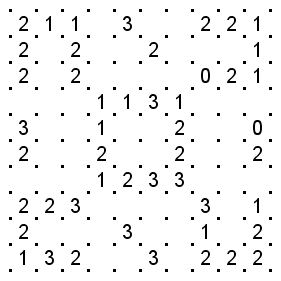
\includegraphics[width =7cm,bb = 0 0 202 202]{sp1slitherlink1.png}
\end{figure}
\Subsection{スリザーリンクのルール}
\begin{description}
\item{1.} 点と点をタテヨコにつなげ、全体で1つの輪っかをつくります。
\item{2.}  4つの点で作られた小さな正方形の中の数字は、その正方形に引く辺の数です。数字のない小さな辺には、何本線を引くかは分かりません。
\item{3.} 線を交差させたり、枝分かれさせたりはしません。
\end{description}
\newpage
\Section{カックロ}
\leavevmode \\
\\

\begin{figure}[H]
\centering 
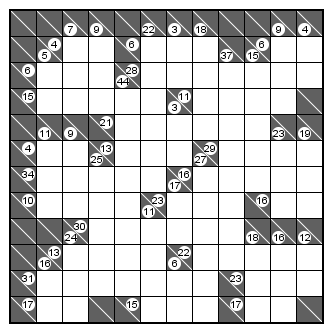
\includegraphics[width = 7cm,bb = 0 0 240 240]{sp1kakkuro1.png}
\end{figure}

\Subsection{カックロのルール}
\begin{description}
\item{1.} すべての白マスに1から9までの数字のどれかひとつを入れます。
\item{2.} ナナメの線の右上の数字は、その右に連続した白マスに入る数字の合計を表し、左下の数字は、その下に連続した白マスに入る数字の合計を表します。
\item{3.} タテヨコへの1つの白マスのつながりには、同じ数字を入れてはいけません。
\end{description}
\Subsection{宣伝文}
SP1といいます。パズルを作りました。息抜きにどうぞ。\\
宣伝ですが、文学部210教室でペンシルパズル同好会の展示を行っています。\\
たくさんのパズルの載った冊子のほか、知恵の輪など触れるパズルも置いています。\\
パズルに興味を持った方はぜひお越しください。
